
\documentclass[12pt,oneside]{book}

\usepackage{caption}
%----------------------------------------------------------------
\usepackage{verbatim}
\usepackage{algorithm}
\usepackage{algpseudocode}
\usepackage{pifont}
\usepackage{amsmath,amsthm,amssymb,amsfonts,multicol}
\usepackage{makeidx}
\usepackage{graphicx}
\usepackage{xcolor}
\usepackage{float}
\usepackage{booktabs}
\usepackage[a4paper,vmargin=3.5cm,left=3cm,right=4cm]{geometry}
\usepackage[colorlinks=true,
	linkcolor=blue!30!black]
	{hyperref}
\usepackage{glossaries}
\usepackage{thesis-utils}
\usepackage[nottoc]{tocbibind}
%----------------------------------------------------------------

%----------------------------------------------------------------
\usepackage[localise=on]{xepersian}
\usepackage{xepersian}
\settextfont[Scale=1.1]{XB Roya}
\setdigitfont[Scale=1]{XB Roya}
%\setlatintextfont[Scale=1]{Tahoma}
%\defpersianfont\Nastaliq[Scale=1.5]{IranNastaliq}
%\defpersianfont\Titre[Scale=1]{XB Titre}

\def\d{\displaystyle}
\def\term{\mathrm{term}}
\allowdisplaybreaks 
%=================================================
\theoremstyle{plain} 
\newtheorem{theorem}{قضیه}[chapter]
\newtheorem{lemma}{لم}[chapter]
\newtheorem{proposition}{گزاره}[chapter]
\newtheorem{corollary}{نتیجه}[chapter]
\newtheorem*{conjecture}{حدس}
\theoremstyle{definition}
\newtheorem{definition}{تعریف}[chapter]
\newtheorem{example}{مثال}[chapter]
\newtheorem{prob}{مساله}[chapter]
\theoremstyle{remark} 
\newtheorem{remark}{ملاحظه}[chapter]
%==================================================
\setcounter{secnumdepth}{3}
%\setcounter{chapter}{4}
\renewcommand{\bibname}{مراجع}
\oddsidemargin =0cm 
\evensidemargin =0cm
\textheight =21cm
\textwidth= 15.3cm
\headsep= 1.2cm
\topmargin  =0cm
\usepackage{perpage}
%\setcounter{chapter}{3}
\MakePerPage{footnote}


% USEFUL COMMANDS
\newcommand{\blankpage}{\thispagestyle{empty}
\begin{center}%
\textit{این صفحه تعمداً خالی گذاشته شده است}%
\end{center}
\clearpage
}

\baselineskip = 1.15cm
\renewcommand{\baselinestretch}{2.3}



\includeonly{
	blank-page,
	logo-pe,
	thanks,
	abstract-pe,
	ch1-preliminaries,
	ch2-background,
	ch3-focused,
	ch4-results,
	appendix,
	abstract-en,
	logo-en
}

\title{پیاده‌سازی روش‌های افزایش وضوح تصاویر با از بین بردن هاله‌های مصنوعی }
\author{منا هادی بر حق طلب}
\captionsetup[lstlisting]{font={small,tt}}

\begin{document}

      \begin{figure}[!htb]
      	\minipage{1\textwidth}
      	\includegraphics[width=\linewidth]{images/besm}
      	
      	\endminipage\hfill
      \end{figure} 

\thispagestyle{empty}
\begin{center}
\vspace{-2cm}
\begin{figure}
\centerline{\includegraphics{images/logo}}
\end{figure}
\makeatletter
{\bf دانشگاه صنعتی شریف  }\\ 
{\bf دانشکده مهندسی کامپیوتر }\vspace{0.3cm}\\
{\bf پایان نامه کارشناسی  }\\ 
{ \bf گرایش مهندسی نرم‌افزار }\\
\vspace{0.4cm}
 عنوان:\\
\vspace{0.3cm}
{\large \bf  \@title}\vspace{1cm}\\

نگارش:\vspace{0.2cm}\\

{\Large \bf \@author}\\
\vspace{0.5cm}
 استاد راهنما: {\Large \bf  آقای دکتر رسول جلیلی }\\
% استاد راهنمای همکار: {\Large \bf  آقای دکتر میرامید حاجی‌میرصادقی}\\
\vspace{0.3cm}
{\large \bf  مهر ۱۳۹۴   }\\
\end{center}
\makeatother
\clearpage
\chapter*{تشکر و قدردانی}
\Huge
با تشکر از اساتيد ارجمند آقايان دکتر جلیلی و بورقانی که در تمام مراحل اين پايان‌نامه هدايت و نظارت خود را از بنده دريغ ننمودند.
\normalsize

\clearpage

{%Open the group
	\makeCondensedChap
	\chapter*{چکیده}
}

شماهای رمزنگاری مبتنی بر نظریه اعداد، همانند  $RSA$ و رمزنگاری بر مبنای خم‌های بیضوی، در صورت تحقق کامپیوترهای کوانتمی، در ابعاد بزرگ می‌شکنند. توسط متخصصان حوزه رمزنگاری ادعا شده‌است، رمزنگاری مشبکه مبنا  یک روش پسا کوانتومی است و در مقابل کامپیوترهای کوانتومی نمی شکند. در رمزنگاری امن-اثبات‌پذیر، امنیت یک شمای رمزنگاری با فرض سخت‌ بودن یک مسئله‌ی ریاضی مشهور اثبات می‌گردد. در رمزنگاری مشبکه مینا، شماهای امن-اثبات پذیر از توزیع گوسی گسسته نمونه‌برداری می‌شود. یکی از عملیات‌های زمان‌بر در شماهای رمزنگاری مشبکه مبنا  نمونه‌برداری  گسسته از  این توزیع است. برای نمونه‌برداری از این توزیع روش‌های متفاوتی وجود دارد. هر کدام از این روش‌ها سرعت و میزان حافظه مصرفی متفاوتی دارند. با توجه به تمایل ما به بهینه بودن این نمونه‌برداری، که باعث بهبود رمزنگاری می‌شود، تلاش است تا سرعت را بالا ببریم و استفاده از حافظه را پایین بیاوریم. در جریان این مصالحه روش  آلیاس در مقابل روش تجمعی - که سریعترین روش استفاده شده در کارهای قبلی مرتبط می‌باشد - از نظر حافظه در یک مرتبه و از نظر سرعت در مرتبه بالاتری قرار دارد . در این مقاله سعی شده است بعد از توضیح کوتاهی در رابطه با مفاهیم اولیه، روش‌های مختلف نمونه‌برداری را توضیح داده و مقایسه‌ای انجام گیرد. در انتها روش آلیاس مورد بررسی قرار می گیرد و نتایج به‌دست‌آمده در مقایسه با روش تجمعی نشان داده می‌شود. 

کلید واژه : رمزنگاری، مشبکه مبنا، توزیع گوسی، توزیع گسسته، تجمعی، آلیاس

\tableofcontents
\listoffigures

%==========================CHAPTERS=======================
\فصل{روش برنولی}

 \begin{figure}[!htb]
 	\minipage{1\textwidth}
 	\includegraphics[width=\linewidth]{images/bernulli1}
 	\caption{توزیع مناسب}\label{fig:adabpted distrbution}
 	\endminipage\hfill
 \end{figure}
 یکی از روش‌های سریع برای نمونه‌برداری روش نمونه‌برداری برنولی است.
در روش برنولی نیاز به نگه داشتن جدول کوچکتر برای اعداد از پیش محاسبه شده داریم ( که سایز آن متناسب لگاریتم $\sigma$  می باشد)
 روش برنولی در حقیقت از روش نمونه‌برداری ردی $(rejection sampling)$ الهام گرفته شده‌است. (شکل ... الف) در روش ردی از توزیع یکنواخت بر روی بازه $[c - \tau _{\sigma} , c + \tau _{\sigma}]$ استفاده می‌شود. مشکل اصلی روش ردی این است که نیازمند محاسبه تابع نمایی با دقت بالا است. در روش برنولی سعی شده است از محاسبه صریح تابع $exp$ جلوگیری شود.
 
 هدف از ارایه روش برنولی آن است که بتوان بدون نگه‌داری جدول‌های بزرگ از پیش محاسبه شده ، و یا محاسبه دقیق تابع توزیع گوسی ، از این توزیع نمونه برداری می کنیم . اولین قدم این است که بتوانیم با کمک توزیع برنولی با بایاس به فرم $exp(-x/f)$ و بدون محاسبه دقیق تابع این کار را انجام دهیم . 
 %%%%%%%%%%%%% inja ro ye check kon%%%%%%%%%%%%%%%%
  دومین قدم این است که بتوانیم توزیع مناسبی را به عنوان ورودی تابع ارایه دهیم تا بتوانیم تعداد رد کردن‌ها را بهینه کنیم.
 
روش تنبل : در روش‌های تنبل ، شیوه‌هایی به کار می رود که محاسبات مورد نیاز برای نتیجه‌گیری را محدود می‌کند. در روش برنولی از این شیوه برای به‌دست آوردن  $a\vee b, a\wedge b$کاربرد دارد که می توان بدون محاسبه $b$ با توجه به مقدار $a$ در خیلی از مواقع جواب را به‌دست آورد. هم‌چنین در هنگام مقایسه دو عدد گاه تنها با مقایسه دو عدد گاه تنها با مقایسه چند بیت پرارزش به جواب دست پیدا کرد.

طبق الگوریتم 8 ..... توزیع برنولی به طور مناسب نمونه برداری کنیم . بنابراین می توانیم از توزیع گوسی با استفاده از یک جدول از پیش محاسبه شده ، نمونه برداری کنیم .
برای به دست آوردن نتیجه مطلوب و راحتی نمونه برداری  از یک توزیع خاص $D_{k, \sigma _{2}}$ استفاده می کنیم. توزیع $D_{k, \sigma _{2}}$ به توزیع نهایی $D_{k\sigma _{2}} $  نسبت به توزیع یکنواخت - که باعث رد شدن نمونه‌های زیادی می شد - نزدیک تر است. 

توزیع گسسته دودویی گوسی :
توزیع گسسته دودویی گوسی $D_{\sigma _{2}} $ را داریم که انحراف معیار آن برابر $\sigma ^{2} _{2}$ و چگالی احتمال آن برابر است با :
  \begin{equation}
\rho _{\sigma _{2}} (x) = e ^{-x^{2}/(2\sigma ^{2} _{2}) = 2^{-x^{2}}      for x \subset \mathbb{Z}
\end{equation}
می خواهیم برای تولید توزیع $D_{k, \sigma _{2}}$ دو توزیع $D_{\sigma _{2}}$  و توزیع یکنواخت را با هم ادغام کنیم.  (عکس ... ب) ما بر قسمت مثبت اعداد تاکید می کنیم  و از نماد $D_{\sigma _{2} ^{+}}$  استفاده می کنیم . الگوریتم ... از فضای $D_{\sigma _{2} ^{+}}$ نمونه برداری می کند .


\section{ مقایسه با سایر روش‌ها}
برتری روش برنولی در مقابل روش تجمعی این است که سایز جدولی که برای انجام عملیات به آن نیاز دارد و باید در حافظه ذخیره کند نسبت به روش تجمعی کمتر است . 







دامنه‌ی دینامیکی\پانوشت{\متن‌لاتین{dynamic range}}
عکس عبارت است از تفاوت مقدار روشنایی بین تاریک‌ترین نقاط و روشن‌ترین نواحی عکس که دارای جزئیات قابل تشخیص باشند. هرچقدر تفاوت این دو مقدار بیشتر باشد، دامنه‌ی دینامیکی عکس بیشتر است. عکسهای
\lr{HDR}\footnote{\lr{High Dynamics Range}}
   عکس‌هایی هستند که از دامنه‌ی دینامیکی بالایی برخوردار هستند، به طوری که هر کانال رنگی آن‌ها می تواند با بیش از 8 بیت نمایش داده می‌شود. 
از طرفی صفحات نمایش عادی قادر به نمایش تمام این دامنه ی روشنایی نیستند. 
هدف اصلی 
\متن‌لاتین{HDR image rendering }
 این است که تصویر‌های 
 \متن‌لاتین{HDR }
 را با استفاده از الگوریتم‌هایی به  گونه ای فشرده سازی کند که تصویر‌هایی که در دستگاه خروجی نمایش داده می شوند، به تصویر واقعی نزدیک تر باشند.
بخش اصلی این کار عبارت است از نگاشت روشنایی عکس‌های با دامنه‌ی دینامیکی بالا به دامنه‌ی دینامیکی دستگاه خروجی که به این کار 
 \متن‌لاتین{tone mapping }
 میگویند.
 
همان طور که در شکل زیر مشاهده می کنید، چشم‌اندازهای طبیعی از دامنه‌ی روشنایی بالایی برخوردار هستند که این دامنه شامل تصویرهای شب‌هنگام، تا تصاویر مناظر طبیعی در روز می شود. برای این که بتوانیم تصویر خوبی از این مناظر ارائه دهیم از عکاسی $HDR$ استفاده می کنیم.
 
 \begin{figure}[!htb]
 	\minipage{1\textwidth}
 	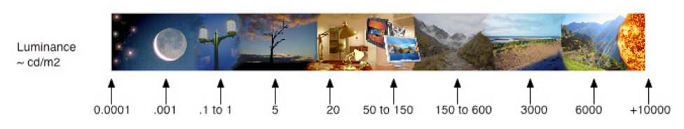
\includegraphics[width=\linewidth]{images/luminancerange}
 	\caption{نمونه‌ای از دامنه‌های روشنایی متفاوت}\label{fig:logtonemap}

 	\endminipage\hfill
 \end{figure}
 


 در این پروژه سعی شده‌است دو  روش  مهم و نسبتا پیچیده برای ارائه‌ی تصویر با دامنه‌ی دینامیکی بالا پیاده‌سازی و مقایسه شوند.
 
 در بخش اول، کلیات این علم و تعریف‌های موجود بررسی می‌شوند. در بخش دوم، تعدادی از الگوریتم‌های پیشین، پیچیدگی و نتایج آنها به اختصار مورد بررسی قرار می گیرند. دربخش سوم، دو روش  مورد نظر در این پروژه توضیح داده می‌شوند، روش پیاده‌سازی آنها شرح داده‌شده، ونتایج بررسی می شوند.
 
 \section{  نگاشت سراسری و نگاشت محلی}
 
نگاشت های سراسری، شامل نگاشت‌هایی است که با توجه به متغیرهای سراسری عکس، مانند میانگین روشنایی انجام می‌شوند. در واقع پس از محاسبه‌ی متغیرهای مطلوب از یک عکس خاص، یک تابع مشخص روی تمام پیکسل‌های عکس اعمال می‌شود. این نوع نگاشت بسیار سریع است. چون معمولا محاسبات پیچیده‌ای ندارند و همچنین می‌توانند با استفاده از
 \متن‌لاتین{look up table  }
ها انجام شوند.

مشکل این نوع نگاشت این است که به دلیل کم کردن تضاد روشنایی باعث از بین رفتن جزئیات یا تغییر رنگ ها می‌شود.

نگاشت‌های محلی، شامل نگاشت هایی است که عملکرد آن روی هر پیکسل، با توجه به متغیرهای احاطه گر آن، متفاوت است.به زبان دیگر پارامترهای تابع، در هر قسمت از تصویر، با توجه به ویژگی‌های آن قسمت از تصویر متفاوت است.

این نوع نگاشت‌ها معمولا دارای محاسبات پیچیده تری هستند، ممکن است هاله‌های مصنوعی ایجاد کنند، و تصویر را کمی تصنعی کنند. اما اگر به درستی اعمال شوند، می‌توانند بهترین تصویر ممکن را ارائه دهند.زیرا سیتستم بینایی انسان به تضادهای روشنایی محلی بیشتر حساس است تا تضادهای سراسری.


\section{تعریف روشنایی در تصاویر رنگی}

روشنایی فضا، روشنایی فیزیکی است و در واقع به معنی شدت انرژی نور است که بر حسب $cd/m^{2}$ قابل اندازه‌گیری است. در تصویر، این روشنایی به صورت مقدار $L$ در فضای  $LUV$ یا به صورت یک ترکیب خطی از کانال‌های رنگ سبز و قرمز و آبی در فضای $RGB$ تعریف می‌شود.

ضرایب این ترکیب خطی به روش‌های گوناگونی قابل تعریف است.  و ممکن است طبق دو تعریف متفاوت، ترتیب روشنایی یک محموعه  تصویر تغییر کند. تفاوت های جزئی  اهمیتی ندارند، چون تعریف دقیق و صحیحی از روشنایی وجود ندارد و این تعریف ها هر چقدر به ذهنیت ما از روشنایی نزدیک تر باشند، بهتر  هستند.

یکی از تعریف‌های متداول به صورت زیر است.

\begin{equation}
luminance = 0.27 red + 0.67 green + 0.06 blue
\end{equation}

\فصل{مقدمه}

رمزنگاری مشبکه مبنا شاخه ای از رمزنگاری که مبتی بر پایه مسایل مشبکه می باشد . برتری که این روش در مقایسه با سایر رمزنگاری های مبتی بر نظریه اعداد نظیر تجزیه و لگاریتم گسسته دارد این است که به نظر می آید یک روش پست کوانتوم است و در مقابل کامپیوترهای کوانتومی نمی شکند . در حالی که رمزنگاری مبتنی بر نظریه اعداد شکسته می شود . همچنین معمولا شماهای این رمزنگاری کارایی بالاتر و سرعت بیشتری دارد.  در رمزنگاری مشبکه مبنا، شماهای امن-اثبات پذیر غالبا از توزیع گسسته گوسی استفاده می کنند . الگوریتم ها و روش هایی که برای نمونه برداری از این توزیع وجود دارد ، محاسبات و / یا حافظه نسبتا زیادی می خواهد. با توجه به استفاده و نیاز فراوان به این نمونه برداری قصد داریم هزینه محاسباتی را بهبود دهیم و پیاده سازی سریعی از آن ارایه دهیم. 


رمزنگاری مشبکه مبنا یکی از اصلی ترین انتخاب‌ها برای رمزنگاری پست کوانتوم است . هیچ الگوریتم کوانتوم بهینه‌ای تاکنون نتوانسته است شمای رمز نگاری مشبکه مبنا را بشکند. بر خلاف شماهایی که به طور گسترده در عمل از آنها استفاده می شود همانند RSA  که شکستن آنها بر مبنای سختی شکستن لگاریتم گسسته است ، هم اکنون می توان با استفاده از کامپیوترهای کوانتومی بزرگ شکسته شود. (514) اثبات امن پذیری شمای مشبکه مبنا در گرو عملیات سنگین و سایز بزرگ کلید است . 
رمز نگاری مشبکه مبنا  به دلیل کاربردهای وسیعش به یکی از مسیرهای تحقیقاتی اصلی در رمزنگاری تبدیل شده‌است)article(

کاربردهای رمزنگاری مشبکه مبنا
رمز نگاری مشبکه مبنا کاربردهای زیادی در امر رمزنگاری دارد. به طور مثال 











\section{نگاشت سراسری}

در نگاشت‌های سراسری همان‌طور که گفته شد، یک تابع مشخص روی تمام پیکسل‌های یک عکس با توجه به متغیرهای عمومی آن اعمال می شود.

\subsection{نگاشت لگاریتمی}
برای محاسبه‌ی تقریبی کدگذاری سیستم بینایی، یک راه حل ساده، استفاده از تابع لگاریتمی است.بنابراین اختلاف واحدها در تصویر با کدگذاری لگاریتمی، نمایشگر اختلاف روشنایی در تصویر است. ایده‌ی اصلی این نگاشت در رابطه ی زیر مشخص شده است. [1] 

در این رابطه$Y$  نشان‌دهنده‌ی روشنایی تصویر، و $D$  نشان‌دهنده‌ی روشنایی دستگاه(صفحه نمایش، چاپگر) است.
میزان روشنایی میانگین تصویر را نیز می‌توان با متغیر $\tau $تغییر داد.

\begin{equation}
Y_{out}  = (D_{max} - D_{min}) \times
 \frac{\log( Y_{in} + \tau) - \log(Y_{min} + \tau)}{\log( Y_{max} + \tau) - \log(Y_{min} + \tau)} 
+ D_{min}
\end{equation}

همان طور که در تصویر مشخسص است ،این نگاشت علی رغم سادگیش، در مقایسه با نگاشت خطی بسیار بهتر عمل  می‌کند.تصویر سمت راست ارائه‌ی عکس با استفاده از نگاشت لگاریتمی، وتصویر سمت چپ، ارائه‌ی همان عکس توسط نگاشت خطی است.
\begin{figure}[!htb]
	\minipage{0.48\textwidth}
	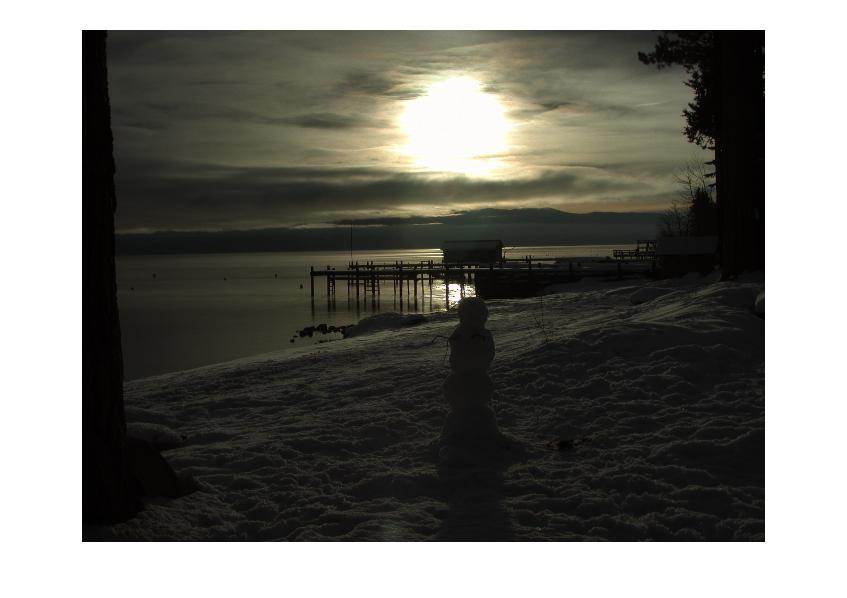
\includegraphics[width=\linewidth]{images/logtonemap}
%	\caption{}\label{fig:logtonemap}
	\endminipage\hfill
	\minipage{0.48\textwidth}
	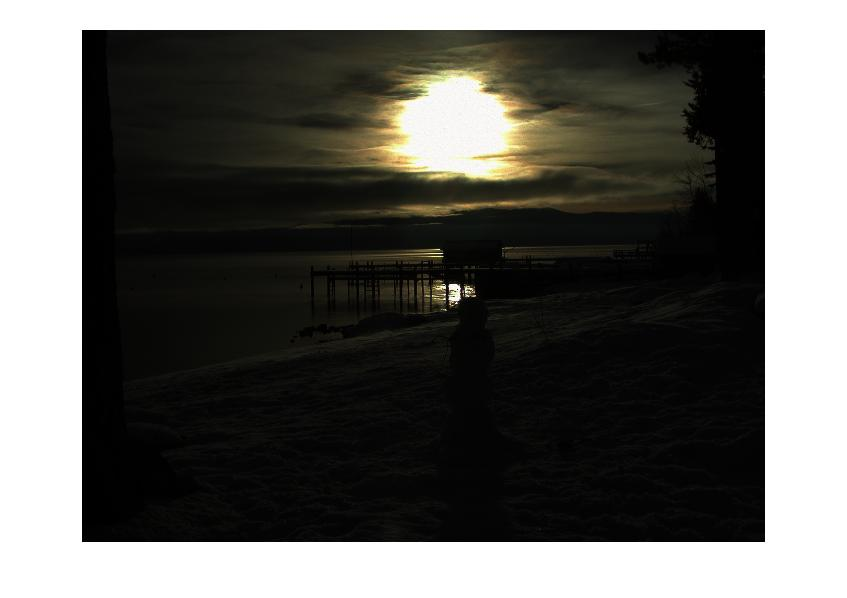
\includegraphics[width=\linewidth]{images/lineartonemap}
	\endminipage\hfill

	\caption{مقایسه‌ی روش‌های
		\متن‌لاتین{tone mapping}: لگاریتمی و خطی
		}\label{fig:linear_vs_log}

\end{figure}

\section{اصلاح نقاط سیاه و سفید}
هر نگاشتی، معمولا شامل این مرحله است که نقاط سیاه عکس را به سیاه، و نقاط سفید تصویر را به سفید نگاشت دهد. در بعضی از نگاشت‌ها مانند نگاشت خطی، این کار خود به خود انجام می‌شود. در غیر این صورت، این کار را پس از نگاشت سراسری انجام می‌دهند تا نتیجه‌ی بهتری بگیرند. در واقع این کار نوعی نگاشت محلی است.

نقاط سیاه و سفید تصویر، به سادگی تیره‌ترین و روشن‌ترین پیکسل‌های تصویر نیستند. زیرا ممکن است به خاطر وجود اختلال، پیکسل‌های پرت داشته باشیم. به همین دلیل، باید گروهی از تیره‌ترین‌ها و گروهی از روشن‌ترین‌ها را پیدا کرد. 
برای این کار می‌توان از روش های هیستوگرام روی 
\متن‌لاتین{luminance image  }
استفاده کرد. به این ترتیب که پیکسل‌های موجود در تصویر را به گروه‌هایی تقسیم کرد که مقدار روشنایی هر گروه، در بازه‌ی مشخصی قرار می گیرد. هر کدام از این بازه ها را 
 \متن‌لاتین{bin  }
 می‌نامیم. 
به این ترتیب، با فرض این که 
 \متن‌لاتین{N}
 تعداد پیکسل‌های موجود در تصویر و 
  \متن‌لاتین{n  }
  تعداد 
  \متن‌لاتین{bin  }
  ها باشد، داریم:

\begin{equation}
N = \sum_{i = 1}^{n} h(i)
\end{equation}
تابع تجمعی 
 \متن‌لاتین{H  }
به شکل زیر تعریف می‌شود، در واقع این تابع نشان دهنده ی مجموع نقاط در بازه های مختلف از 1 تا یک بازه ی خاص 
\متن‌لاتین{j  }
است.:
\begin{equation}
H(j) = \sum_{j^{'} = 1}^{j} h(j^{'})
\end{equation}

\متن‌لاتین{H  }
 یک تابع اکیدا صعودی است. نقاط  سیاه  و سفید 
 \متن‌لاتین{w, b  }
 را به ترتیب نقاطی که در یک درصد ابتدای این تابع قرار می‌گیرند، و نقاطی که در یک درصد آخر قرار می‌گیرند تعریف می‌کنیم.

حال برای اصلاح تصویر، کافی است نقاط سیاه را به 0، نقاط سفید را به 1، و بقیه ی نقاط را به  صورت خطی به  بازه‌ی [0,1]  نگاشت داد. این کار از طریق رابطه ی زیر انجام می شود. قابل ذکر است که طی این تساوی هر کانال رنگ 
\متن‌لاتین{c  }
به بازه ی [0,1] نگاشت می شود.
\begin{equation}
I_{new} = min(1, \frac{max(0, I_{c}(p) - b)}{w - b})
\end{equation}
در تصویر
\ref{fig:bwcorrection}
 یک تصویر سیاه و سفید و در تصویر 
\ref{fig:bwcorrection2}
  یک تصویر رنگی  را قبل و بعد از اصلاح نقاط سیاه و سفید آن مشاهده می کنید.
\begin{figure}[!htb]
 		\minipage{1\textwidth}

 		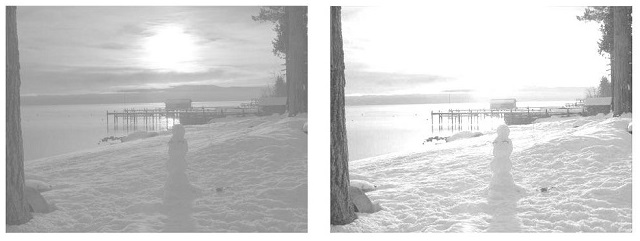
\includegraphics[width=\linewidth]{images/bwcorrection}

 		\caption

 		[حاصل اجرای الگوریتم اصلاح نقاط سیاه و سفید]
 		{
حاصل اجرای الگوریتم اصلاح نقاط سیاه و سفید: عکس سمت راست اصلاح شده‌ی عکس سمت چپ است
}\label{fig:bwcorrection}
 		\endminipage\hfill

 		
 %	\centerline{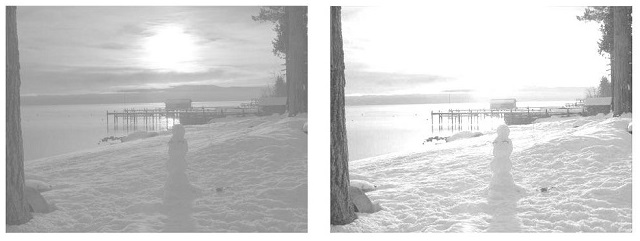
\includegraphics{images/bwcorrection}}
\end{figure}
 \begin{figure}[!tb]
 		\minipage{1\textwidth}

 		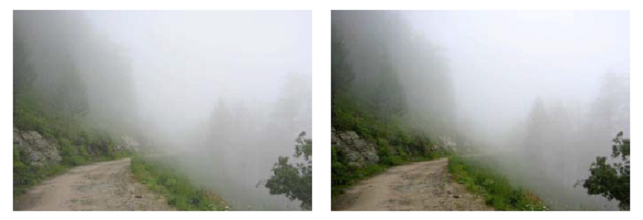
\includegraphics[width=\linewidth]{images/bwcorrection2}

 	\caption
 	[حاصل اجرای الگوریتم اصلاح نقاط سیاه و سفید بر روی عکس رنگی]
{حاصل اجرای الگوریتم اصلاح نقاط سیاه و سفید بر روی عکس رنگی: عکس سمت راست اصلاح شده‌ی عکس سمت چپ است}
 	\label{fig:bwcorrection2}
 	\endminipage\hfill
 %	\centerline{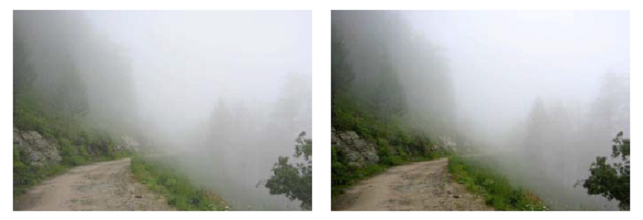
\includegraphics{images/bwcorrection2}}
 \end{figure}
\فصل{الگوریتم‌های پیاده سازی شده}

\section{نگاشتی بر اساس سیستم بینایی انسان}
سیستم بینایی انسان، برای دیدن جزئیات در نورهای مختلف، و ساخت یک تصویر درست در ذهن
\lr{ذهن}\footnote{\lr{percept}}
، به روش های مختلفی خود را سازگار می کند.
 در این روش سعی می کنیم برای نزدیک کردن تصویر خروجی به تصویر واقعی یا تصویری که چشم ما از منظره درک می کند، سازگاری های انجام شده توسط سیستم بینایی انسان را توسط کامپیوتر شبیه سازی کنیم. 
 
 اولین مرحله‌ی سازگاری در سیستم بینایی، در مردمک چشم صورت می‌گیرد که اندازه ی خود را با توجه به میزان روشنایی کلی که وارد چشم می‌شود تنظیم می کند. در مرحله‌ی دوم، شبکیه‌ی چشم میزان حساسیتشان را به میانگین روشنایی وارده تغییر می دهند. در مرحله ی سوم، یک سازگاری محلی برای مشخص کردن تضاد به وجود آمده در قسمت‌های متفاوت تصویر با توجه به محل خیره شدن انجام می شود.
 
در این بخش روشی برای ارائه‌ی تصاویر با دامنه‌ی دینامیکی بالا ارائه می شود، که برگرفته از نگاشت‌های سراسری و محلی‌ای است که در سیستم بینایی انسان انجام می شود. 

از مزایای این روش، استفاده از نگاشت محلی با توجه به شکل لبه‌های با تضاد روشنایی بالا است. این موضوع خود باعث کاهش هاله های مصنوعی که در اثر نگاشت‌های محلی به وجود می‌آید می‌شود.
همچنین در این روش،  روشنایی تصویر  چداگانه پردازش می شود. برای این کار روشنایی را با استفاده از آنالیز مولفه‌های اصلی محاسبه می کنیم که تعامد روشنایی و کانال‌های رنگ را به حداکثر برسانیم. در نتیجه، در اثر این نگاشت، تغییر رنگ کمتری در تصویر ایجاد می شود.

کلیات این نگاشت به این صورت است که ابتدا تصویر روشنایی را تفکیک می کنیم. روی تصویر روشنایی، یک مرحله نگاشت سراسری، و پس از آن یک نگاشت محلی اجرا می کنیم. به صورت موازی، روی تصویر رنگی نیز یک نگاشت سراسری اجرا می کنیم. و در نهایت این دو تصویر را با هم ترکیب می کنیم.
\begin{figure}[!htb]
	\minipage{1\textwidth}
	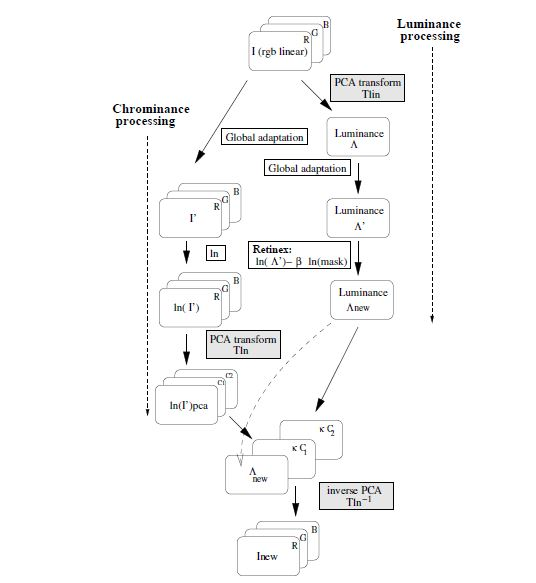
\includegraphics[width=\linewidth]{images/retinexbigpic}
	\caption{}\label{fig:logtonemap}
	\endminipage\hfill
	%	
	%	\centerline{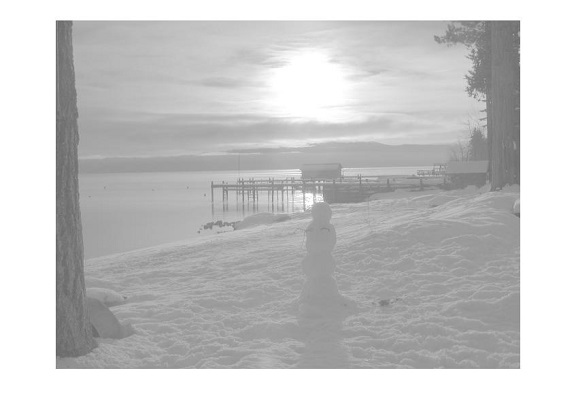
\includegraphics{images/retinexglobal}}
\end{figure}

در این بخش به مراحل پیاده سازی و اچرای این الگوریتم می پردازیم.

\subsection{نگاشت سراسری}
در این قسمت، فشرده‌سازی اولیه ی دامنه، روی تصویر اجرا می‌شود، این فشرده‌سازی، در واقع کاری که مردمک چشم انجام می‌دهد را شبیه سازی می‌کند.این شبیه‌سازی، می‌تواند توسط یک تابع نمایی انجام شود.انحنا‌ی تابع نمایی‌ای که این نگاشت را تقریب می‌زند، به میانگین روشنایی عکس وابسته است.

برای محاسبه‌ی روشنایی، از اولین مولفه‌ی اصلی که روی محور 
\متن‌لاتین{RGB }
 به دست می‌آید استفاده می کنیم. به این ترتیب، روشنایی بیشترین استقلال ممکن را نسبت به رنگ‌ها دارد، و پردازش روشنایی مستقل از رنگ‌ها به خوبی انجام می‌شود.
 
 \begin{code}
 \begin{matlab}
 	 flatimage = reshape(image, [N 3]);
 	 coeff = princomp(flatHDR);
 	 PsiCoeff = [coeff(:, Gcoeff)];
 	 Psi = zeros(n, m);
 	 %R,G and B are first, second, and thired column of HDR image
 	 %representing red, green and blue channels respectively
 	 Psi(:,:) = R * PsiCoeff(1, 1) + G * PsiCoeff(2, 1) + B * PsiCoeff(3, 1);
 \end{matlab}
 %\caption{نمونه کد متلب}
 \end{code}


اکنون $\Lambda$ روشنایی محاسبه شده برای عکس توسط مولفه‌ی اصلی تصویر
\متن‌لاتین{RGB }
است. میانگین روشنایی از طریق رابطه‌ی زیر قابل محاسبه است که در آن $N$ تعداد پیکسل‌های موجود در تصویراست.

\begin{equation}
	\Lambda_{av} = \frac{\varSigma ln(\Lambda(p))}{N}
\end{equation}

روشنایی نهایی، از طریق رابطه‌ی زیر قابل محاسبه است.

\begin{equation}
	\Lambda^{'}(p) = \Lambda^{\frac{1}{\gamma}}	
\end{equation}

$\frac{1}{\gamma}$
در رابطه ی بالا،  یک تابع مستوی از  روشنایی میانگین است که از طریق زیر به دست می آید. این ضرایب به صورت تجربی به دست آمده اند.

\begin{equation}
	\frac{1}{\gamma} = min(1, \frac{1}{6} \Lambda_{av} + \frac{1}{3})
\end{equation}

تصویر زیر، توسط این نگاشت به وجود آمده است. همان طور که می بینید، در تصویر بخش های سفید و سیاه، به خوبی نشان داده نشده اند. البته رنگی نبودن آن، به خاطر این است که در این نگاشت فقط روشنایی عکس را مورد پردازش قرار داده ایم.

 
 \begin{figure}[!htb]
 		\minipage{1\textwidth}
 		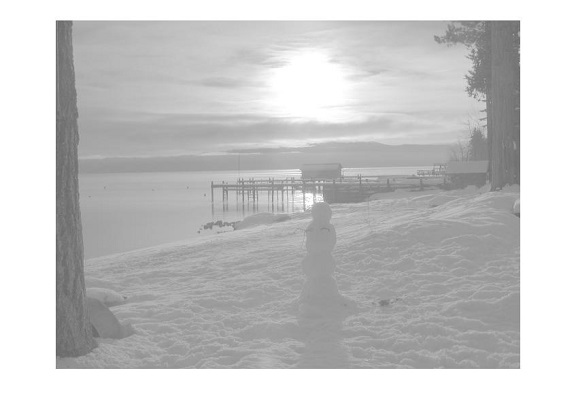
\includegraphics[width=\linewidth]{images/retinexglobal}
 		\caption{}\label{fig:logtonemap}
 		\endminipage\hfill
 		%	
 %	\centerline{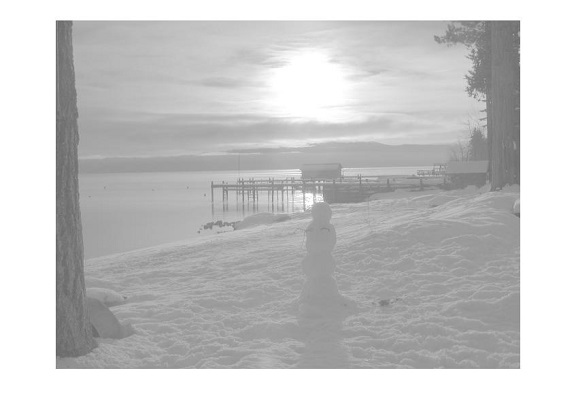
\includegraphics{images/retinexglobal}}
 \end{figure}
 
 
\subsection{نگاشت محلی}

پس از نگاشت سراسری که روی تصویر انجام می‌شود، یک نگاشت محلی برای افزایش وضوح جزئیات صورت می‌گیرد.

نگاشت محلی که در این الگوریتم در نظر گرفته شده، یک نگاشت 
\متن‌لاتین{surround-based }
  است، به  این معنی که به هر پیکسل، یک مقدار جدید، با توجه به پیکسل‌های احاطه‌گر آن اختصاص می دهد.معمولا در این الگوریتم‌ها از اختلاف بین مقدار هر پیکسل، و یک ماسک که میانگین وزن‌دار پیکسل‌های احاطه گر آن است، استفاده می‌شود.
  


\begin{equation}
	\Lambda^{"} = ln(\Lambda^{'}(p)) - ln(mask(p))
\end{equation}

\subsubsection{اصلاح بخش سیاه و سفید}
امامشکل این رابطه، این است که بخش‌های سیاه تصویر، کاملا سیاه نمی‌مانند، و بخش‌های سفید نیزکمی تیره می‌شوند.برای رفع این مشکل، یک متغیر $ \beta$ تعریف می‌کنیم، که این تبدیل‌ رابهبود ببخشد.


\begin{equation}
	\Lambda^{"} = ln(\Lambda^{'}(p)) - \beta ln(mask(p))
\end{equation}

رای محاسبه‌ی این رابطه، با توجه به این که $mask$ و $\Lambda$ هر دو در بازه‌‌ی [0,1] هستند، آن‌ها را به مقیاس [0.1,100] نگاشت می‌دهیم , مقادیر جدید آن ها را به ترتیب $mask_{ln}$ و $\Lambda^{'}_{ln}$ می نامیم. این مقادیر از طریق روابط زیر قابل محاسبه اند. البته لگاریتم طبیعی در بازه ی مشخص شده، از طریق تابع نمایی $\frac{1}{3}$ نیز قابل تقریب زدن است.


\begin{equation}
	\Lambda^{'}_{ln} = \frac{1}{ln(100)}.ln(max(0.1, \Lambda^{'}(p)\times 100))
\end{equation}	

\begin{equation}	
	mask^{'}_{ln} = \frac{1}{ln(100)}.ln(max(0.1, mask^{'}(p)\times 100))	
\end{equation}

به این ترتیب، رابطه‌ی فوق به شکل زیر بازنویسی می‌شود.


\begin{equation}
	\Lambda^{"} = \Lambda^{'}_{ln}(p) - \beta mask_{ln}(p)
\end{equation}
حال به ضریب بتا می‌پردازیم.
این ضریب به  صورت یک تابع سیگموئید و به گونه‌ای تعریف شده‌است که برای مقادیر با روشنایی شدید، ضریب نزدیک به صفر باشد، تا با کم شدن مقدار 
\متن‌لاتین{$ \beta mask_{ln}(p) $ }
از مقدار خود پیکسل، روشنایی کمتر نشود. همچنین برای مقادیر با روشنایی کم، این ضریب نزدیک به یک می‌باشد که به این ترتیب، این مقدار، همچنان تیره می‌ماند. این ضریب، از طریق رابطه زیر قابل محاسبه است.


\begin{equation}
	\beta = 1 - \frac{1}{1 + e^{-10.(max(0, \Lambda^{'}_{ln}(p)) - 0.5))}}
\end{equation}

حال باید اعداد را به مقیاس اصلی باز گردانیم، ضمنا با توجه به این که ممکن است در این میان عددی منفی شود، طبق بحث صورت گرفته در بخش 2.2، رابطه‌ی بالا را به صورت زیر اصلاح می‌کنیم.

\begin{equation}
	\Lambda_{new} = min(1, \frac{max(0, \Lambda^{"}(p) - b)}{\omega - b}) 
\end{equation}

\subsubsection{معضل هاله‌های مصنوعی  }

یکی دیگر از معضلات این روش، معضل انتخاب بین ارائه‌ی خوب تصویر، و افزایش وضوح جزئیات در تصویر است. اگر پیکسل‌های احاطه‌گر را کوچک در نظر بگیریم، به صورت محلی وضوح تصویر بالا می‌رود، اما باعث ایجاد هاله‌های مصنوعی می‌شود.استفاده از فضای احاطه‌گر بیشتر، هاله‌های مصنوعی را کاهش می‌دهد، اما تضادها را کاهش داده، و در نتیجه وضوح تصویر را کاهش می‌دهد.
در این الگوریتم، برای مقابله با مشکل هاله‌های مصنوعی، فضای احاطه‌گر را ثابت در نظر نگرفته، و آن راسازگار با لبه‌های با تضاد روشنایی شدید تعریف می‌کنیم. به این ترتیب، بخش‌های روشن نامربوط، روی روشنایی بخش‌های تاریک تصویر تاثیرگذار نمی‌شوند و بالعکس. 
برای مشخص کردن گوشه‌ها، از الگوریتم $canny$ استفاده می‌کنیم.

با توجه به مطرح شدن گوشه‌ها،  محاسبه‌ی $mask$ برای هر کدام از پیکسل‌ها باید به صورت جداگانه صورت گیرد. به طور کلی $mask$ میانگین وزن‌دار میزان روشنایی فضای احاطه‌گر تعریف شده برای هر پیکسل است. این مقدار از طریق رابطه‌ی زیر قابل محاسبه است. 

\begin{equation}
	mask(x,y) = \frac
	{\sum_{\theta=0}^{360}\sum_{r=0}^{r_{max}}
		\Lambda'\big(x+r.\cos(\theta), y+r.\sin(\theta) \big).e^{-\frac{r^2}{\sigma_{\theta,r}^2}}}
	{\sum_{\theta=0}^{360}\sum_{r=0}^{r_{max}}e^{-\frac{r^2}{\sigma_{\theta,r}^2}}}
\end{equation}

 
 که در آن 
 \متن‌لاتین{(x,y) }
 نشان‌دهنده‌ی مختصات پیکسل
  \متن‌لاتین{p } ، 
  \متن‌لاتین{$ \theta $ }
 زاویه‌ای که یک پیکسل در فضای احاطه‌گر با 
  \متن‌لاتین{p } 
 می‌سازد، و 
  \متن‌لاتین{r }
 فاصله  با
  \متن‌لاتین{p } 
   است.
 
 همچنین مقدار  
   \متن‌لاتین{$\sigma$}
  در صورتی که  یک گوشه با تضاد روشنایی بالا از آن عبور نکرده باشد، برابر با 
   \متن‌لاتین{$\sigma_{0}$}
   و در غیر این صورت برابر با 
   \متن‌لاتین{$\sigma_{1}$}
   است.
این مقادیر به صورت تجربی برابر $\frac{1}{16} $و $\frac{1}{8} $در نظر گرفته می شوند.
 %todo
 
 \subsubsection{یافتن لبه‌ها }
 
 همان‌طور که پیش تر گفته شد، برای یافتن لبه‌ها با تضاد روشنایی بالا، از الگوریتم 
  \متن‌لاتین{canny }
 استفاده می‌کنیم.
 این الگوریتم لبه‌ها را با توجه به بیشینه‌های محلی شیب تصویر، پیدا می‌کند. لبه‌های ضعیف و قوی را مشخص می‌کند. اگر لبه‌ای ضعیف باشد، تنها در صورتی آن را نمایش می‌دهد که به یک لبه‌ی قوی متصل باشد. آستانه‌ای که تفاوت لبه‌ی ضعیف و قوی را مشخص کند، در تمام تصویر‌ها یک مقدار ثابت است که به صورت تجربی به دست آمده است. به این ترتیب، ممکن است برای تصویر‌هایی که لبه‌ای با تضادروشنایی نسبتا بالا ندارند، هیچ لبه‌ای تشخیص داده نشود.
 در پایین، چند نمونه از تصاویر سیاه و سفید و لبه های تشخیص داده شده برای آن ها با الگوریتم 
   \متن‌لاتین{canny }
 را مشاهده می کنید. همان طور که گفته شد، الگوریتم مورد بحث، روشنایی را از رنگ جدا می کند، در نتیجه به طور خودکار در این مرحله، تصویری که داریم سیاه و سفید است.
  \begin{figure}[!htb]
  		\minipage{1\textwidth}
  		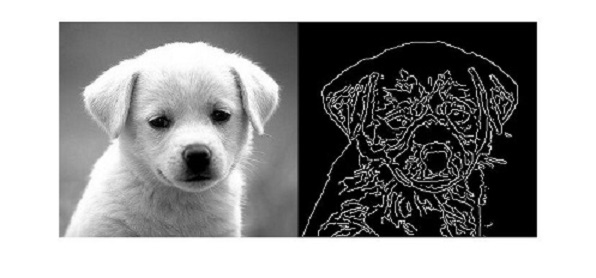
\includegraphics[width=\linewidth]{images/cannyexample1}
  		\caption{}\label{fig:logtonemap}
  		\endminipage\hfill
  %	\centerline{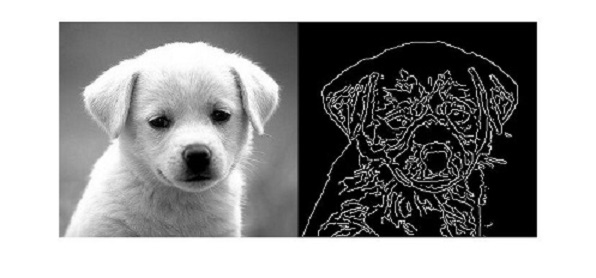
\includegraphics{images/cannyexample1}}
  \end{figure}
  
   
   \begin{figure}[!htb]
   		\minipage{1\textwidth}
   		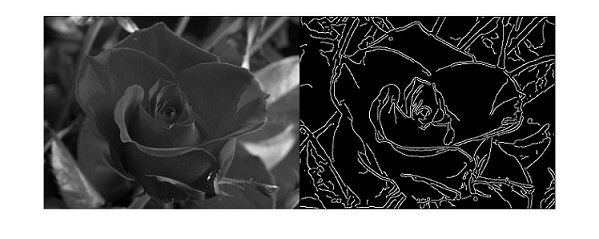
\includegraphics[width=\linewidth]{images/cannyexample2}
   		\caption{}\label{fig:logtonemap}
   		\endminipage\hfill
  % 	\centerline{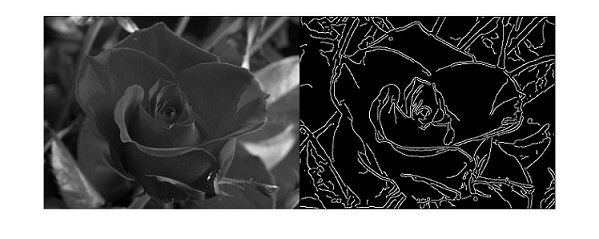
\includegraphics{images/cannyexample2}}
   \end{figure}
   
 
\subsection{پردازش رنگ}
برای پردازش رنگ تصویر، دقیقا مراحلی که در پردازش تصویر روشنایی انجام دادیم را روی هر کدام از کانال‌های رنگی تکرار می‌کنیم، با این تفاوت که نگاشت محلی را انجام نمی‌دهیم.

نگاشت سراسری ای که در بخش قبل گفته شد روی هر کدام از 
 \متن‌لاتین{R }،
  \متن‌لاتین{G } و 
   \متن‌لاتین{B }
 تصویر 
    \متن‌لاتین{I }
  اجرا می‌شود تا تصویر 
     \متن‌لاتین{$I^{'}$ }
  ایجاد شود.
  از مقادیر لگاریتم می‌گیریم . اولین مولفه‌ی اصلی این مقادیر را محاسبه می کنیم تا 
$\ln(I')_{pca}$              
    به دست بیاید. این مقدار را با
$\Lambda_{new}$
   جایگذاری می کنیم. همان طور که قبل تر هم اشاره شد، مولفه ی اول $PCA$ نمایش گر نور، و مولفه های دوم و سوم، به ترتیب نمایشگر زرد -آبی  و قرمز-سبز هستند.
   
   حال تصویر را باز سازی می کنیم. 
   برای این کار  ماتریس تصویر را در فضای $PCA$به شکل زیر می‌سازیم.
   
   ستون اول ماتریس، روشنایی تصویر است که در بخش قبل محاسبه شد. ستون دوم و سوم به ترتیب مولفه‌های دوم و سوم $PCA$ هستند. حال کافی است از یک تبدیل برای انتقال تصویر از فضای $PCA$ به فضای $RGB$ استفاده کرد تا تصویر نهایی در قالب $RGB$ ایجاد شود.
   
    
    \begin{code}
    	\begin{matlab}
    		 % change matrix represenation into vector representation
    		 b1 = PCA(:,:,1);
    		 b2 = PCA(:,:,2);
    		 b3 = PCA(:,:,3);
    		 b_vec = cat(2,b1(:),b2(:),b3(:));	 
    		 % apply transformation
    		 RGB_vec = b_vec*inv(V);
    	\end{matlab}
    	%\caption{نمونه کد متلب}
    \end{code}
    
  
  

\section{نگاشت 
	\متن‌لاتین{reinhard }
}

در این روش، ابتدا یک نگاشت اولیه‌ی سراسری اعمال می‌کنیم. این نگاشت با استفاده از سیستم zone که در ادامه تعریف می‌شود انجام می‌شود. پس از این نگاشت، در صورت نیاز، یک اصلاح محلی به نام  dodging and burning انجام می‌شود.
%todo


\subsection{نگاشت سراسری}
کلید یک تصویر، نشان‌دهنده‌ی ذهنیت ما نسبت به میزان روشنایی کلی یک تصویر است. به عنوان مثال برای یک دیوار سفید، دارای مقدار کلید بالا، و مقدار کلید یک دیوار سیاه، کوچک است.
یک روش ساده برای توصیف این مقدار استفاده از کدگذاری
\متن‌لاتین{log-average luminance }
است، که از طریق رابطه‌ی زیر قابل مقایسه است.

\begin{equation}
	\overline L_{w} = \frac{1}{N} \exp (\sum_{x,y} \log(\sigma + L_{w}(x,y))) 
\end{equation}

در این رابطه، 
\متن‌لاتین{L(x,y)}
میزان روشنایی تصویر در پیکسل 
\متن‌لاتین{(x,y) }
است، و $\sigma$ یک مقدار کوچک است که برای جلوگیری از یکپارچه شدن تصویر اضافه می‌شود. این یکپارچگی رنگ، در صورت وجود نقاط سیاه در تصویر به وجود می‌آید.
خواسته‌ی ما این است که پیکسل با روشنایی میانگین( که در بالا محاسبه شده است) را به $middle-gray$ یا مقدار 0.18 نگاشت دهیم. به این ترتیب رابطه‌ی زیر را داریم. 

\begin{equation}
	L(x,y) = \frac{a}{\overline{L_{w}}}L_{w}(x,y)
\end{equation}

با تغییر مقدار   $a$ می‌توان میزان روشنایی را تغییر داد، این میزان را کاربر می‌تواند خود انتخاب کند، زیرا همان طور که مشخص است، نگاشت صحیح، معنی ندارد و به هر میزان که کاربر احساس بهتری داشته باشد، نگاشت بهتر است. ما برای پیاده سازی همان طور که گفته شد، مقدار آن را برابر 0.18 قرار دادیم.

تصاویر 3.1 این نگاشت را با استفاده از مقادیر مختلف $a$ نشان می دهد.

\begin{figure}[!htb]
	\minipage{1\textwidth}
	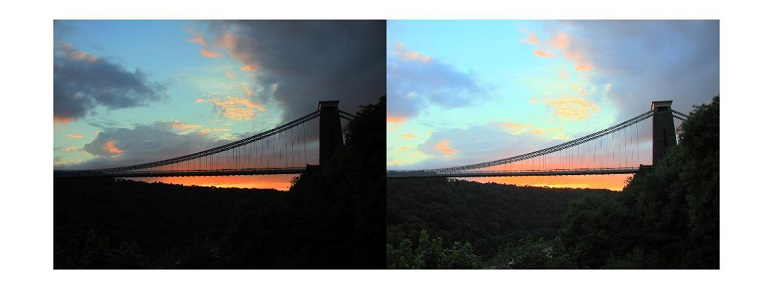
\includegraphics[width=\linewidth]{images/reinharda}
	\caption{}\label{fig:logtonemap}
	\endminipage\hfill
	%	\centerline{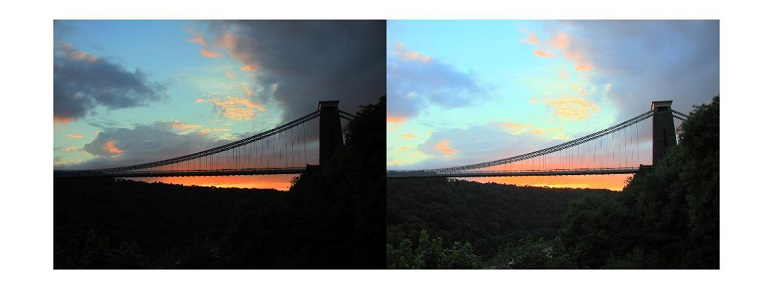
\includegraphics{images/reinharda}}
\end{figure}


نکته‌ای که وجود دارد این است که این گونه خطی نگاشت دادن روشنایی‌ها، عملکرد خوبی ندارد، زیرا تصاویر معمولا دارای رنج روشنایی متوسط هستند که در نقاط خی کمی، روشنایی‌شان از بازه‌ی عادی می‌گذرد. برای حل این مشکل، رابطه‌ی زیر را پیشنهاد می‌کنیم.

\begin{equation}
	L_{d}(x,y) = \frac{L(x,y) (\frac{1+L(x,y)}{L^{2}_{white})}}{1 + L(x,y) }
\end{equation}

که در این رابطه $ L_{white}$کوچک‌ترین مقداری است که می‌خواهیم مقادیر بزرگ تر از آن به سفید نگاشت شوند.

اگر مقدار  $ L_{white}$ را برابر با بی نهایت قرار دهیم، 
\متن‌لاتین{burning } 
اتفاق میفتد. اما اگر مقدار آن را برابر با بیشترین مقدار روشنایی موجود در تصویر قرار دهیم، این مشکل نیز حل می‌شود.

تصاویر 3.2، این نگاشت را با استفاده از مقادیر مختلق برای 
$ L_{white}$ 
نشان می دهد.

\begin{figure}[!htb]
	\minipage{1\textwidth}
	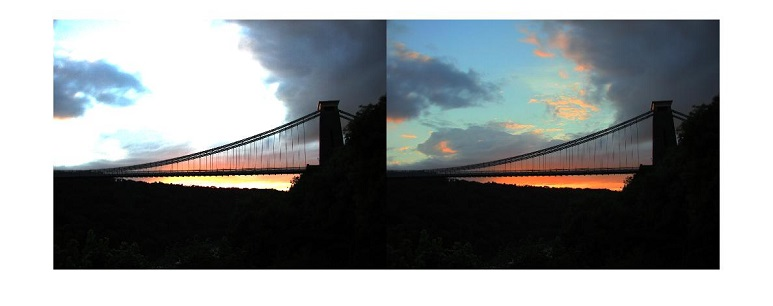
\includegraphics[width=\linewidth]{images/reinhardw}
	\caption{}\label{fig:logtonemap}
	\endminipage\hfill
	%	\centerline{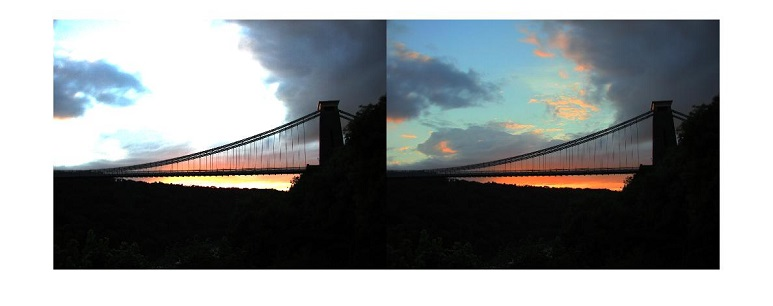
\includegraphics{images/reinhardw}}
\end{figure}


  
 \subsection{نگاشت محلی}
  

\فصل{روش آلیاس}
\lr{آلیاس}\footnote{\lr{alias}
این روش ، یک روش برای تولید کردن یک عدد تصادفی$x$ با داشتن یک بردار احتمال$ p_{0}, p_{1}, ..., p_{k}$  می‌باشد   . در این روش به یک جدول با اندازه$ O(K)$  نیاز داریم.  زمان مورد نیاز این روش  بعد از  انجام پیش محاسبات $ O(1)$ می باشد.
 این روش بر تئوری زیر استوار است :
هر بردار احتمال p_{0}, p_{1} , ..., p_{k -1}  را می توان به صورت مجموعه ای از زوج مرتب ها نمایش داد . 


در زیر چند تصویر که با استفاده از روش‌های مختلف بحث شده در این پروژه ساخته شده اند را مشاهد می‌کنید.

  
  \begin{figure}[!htb]
  	\minipage{0.48\textwidth}
  	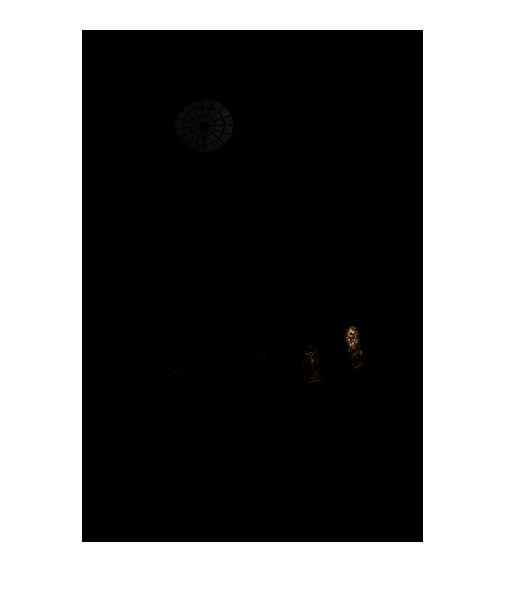
\includegraphics[width=\linewidth]{images/linearhdr1}
  	\caption{linear}\label{fig:logtonemap}
  	\endminipage\hfill
  	\minipage{0.48\textwidth}
  	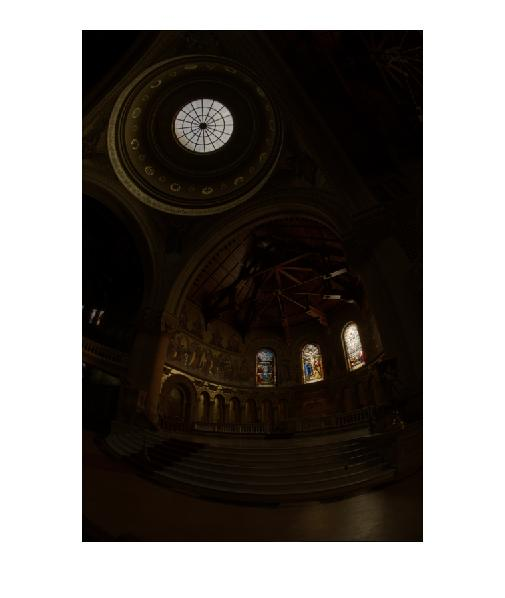
\includegraphics[width=\linewidth]{images/loghdr1}
  	\caption{logarithmic}\label{fig:lineartonemap}
  	\endminipage\hfill
  	% 	\centerline{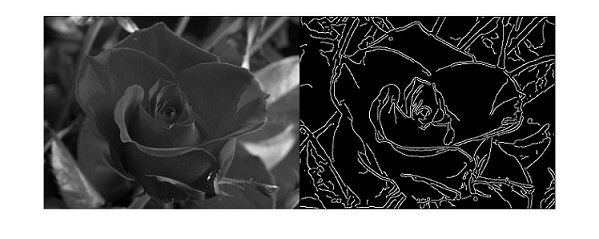
\includegraphics{images/cannyexample2}}
   \end{figure}
      
  \begin{figure}[!htb]
    \minipage{1\textwidth}
      	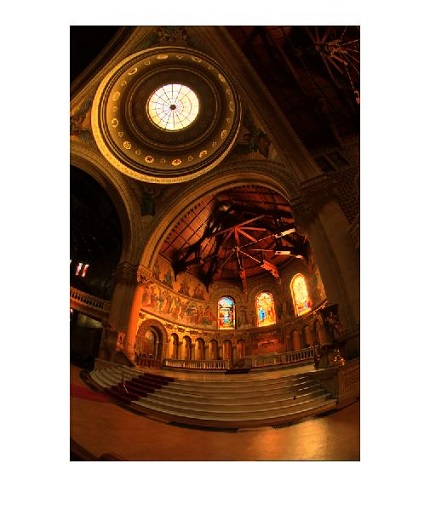
\includegraphics[width=\linewidth]{images/reinhardhdr1}
      	\caption{rainhard}\label{fig:logtonemap}
    \endminipage\hfill
      	% 	\centerline{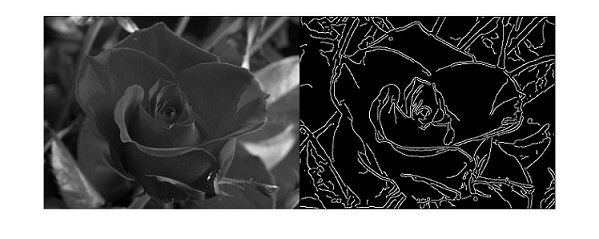
\includegraphics{images/cannyexample2}}
   \end{figure}
      
        
    \begin{figure}[!htb]
     \minipage{1\textwidth}
        	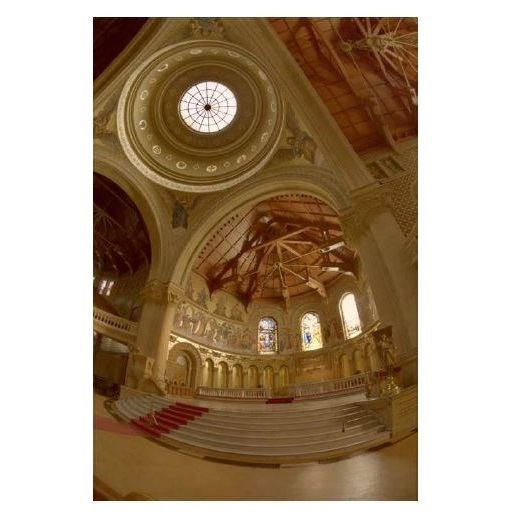
\includegraphics[width=\linewidth]{images/retinex3}
        	\caption{retinex}\label{fig:logtonemap}
      \endminipage\hfill
        	% 	\centerline{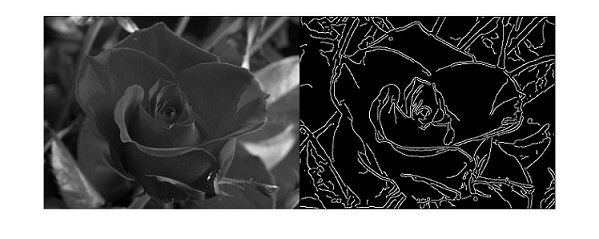
\includegraphics{images/cannyexample2}}
    \end{figure}
        
        
      \begin{figure}[!htb]
      	\minipage{0.48\textwidth}
      	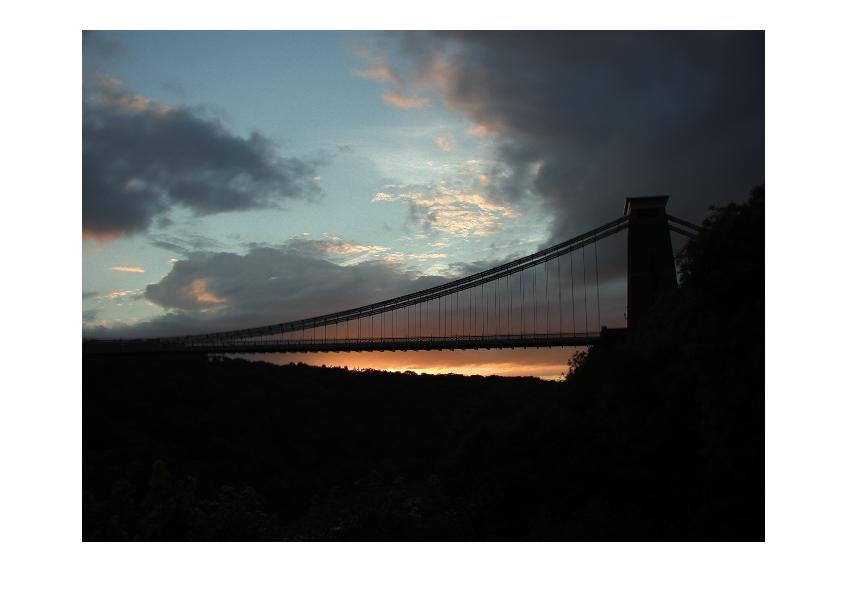
\includegraphics[width=\linewidth]{images/linearhdr3}
      	\caption{linear}\label{fig:logtonemap}
      	\endminipage\hfill
      	\minipage{0.48\textwidth}
      	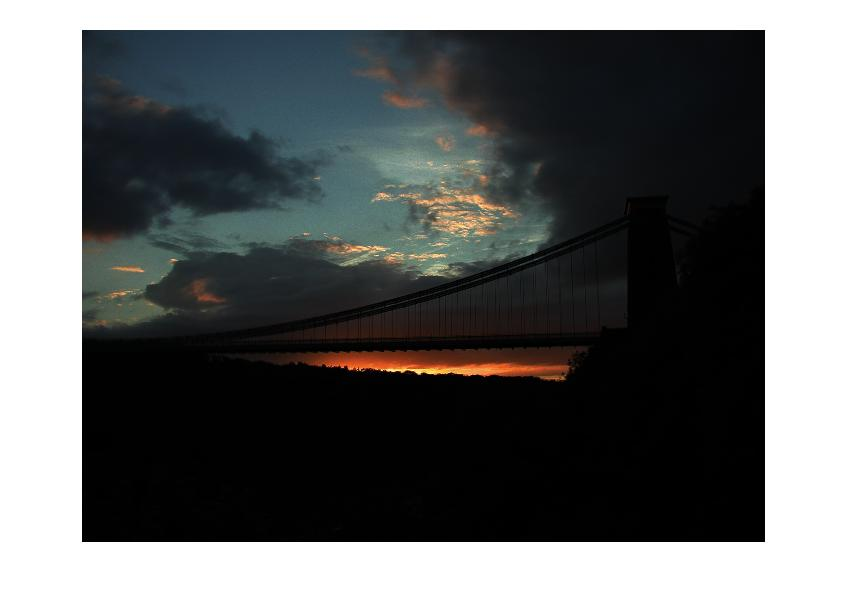
\includegraphics[width=\linewidth]{images/loghdr3}
      	\caption{logarithmic}\label{fig:lineartonemap}
      	\endminipage\hfill
      	% 	\centerline{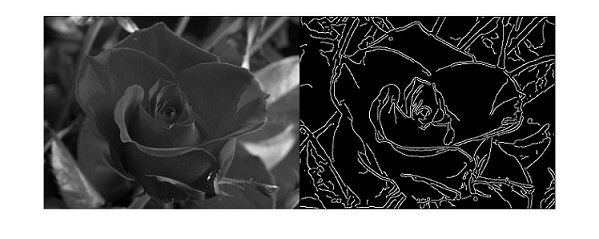
\includegraphics{images/cannyexample2}}
      \end{figure}
      
      \begin{figure}[!htb]
      	\minipage{1\textwidth}
      	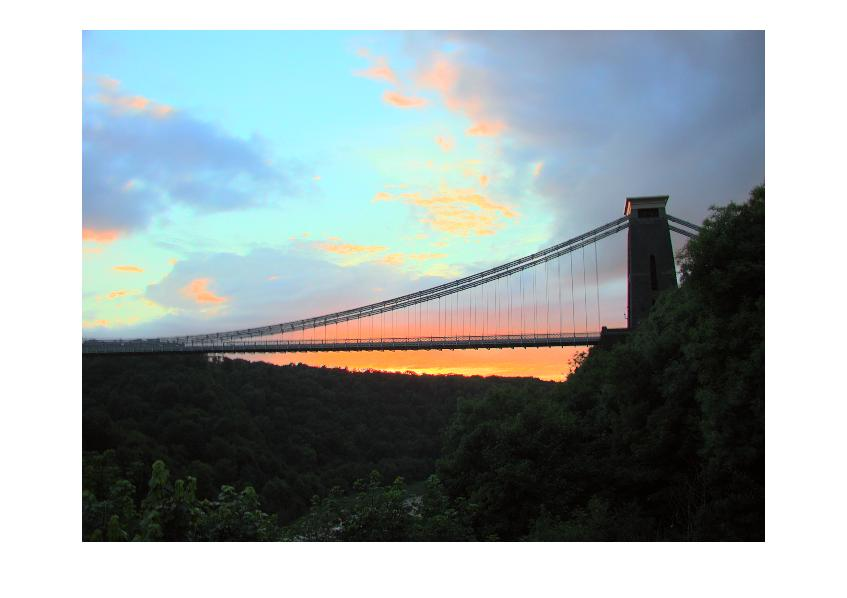
\includegraphics[width=\linewidth]{images/rainhardhdr3}
      	\caption{rainhard }\label{fig:logtonemap}
      	\endminipage\hfill
      	% 	\centerline{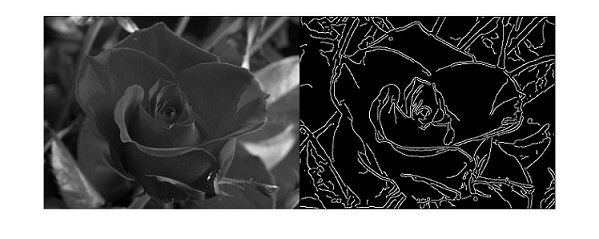
\includegraphics{images/cannyexample2}}
      \end{figure}
      
      
      \begin{figure}[!htb]
      	\minipage{1\textwidth}
      	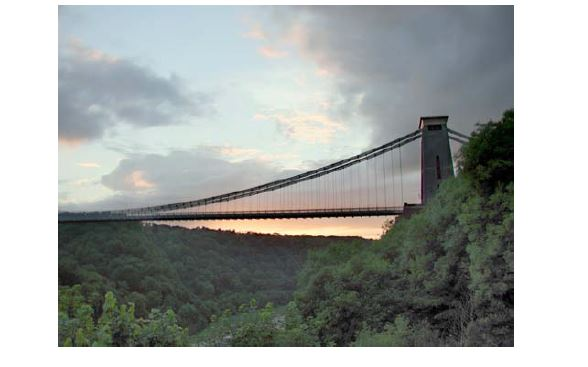
\includegraphics[width=\linewidth]{images/retinex1}
      	\caption{retinex}\label{fig:logtonemap}
      	\endminipage\hfill
      	% 	\centerline{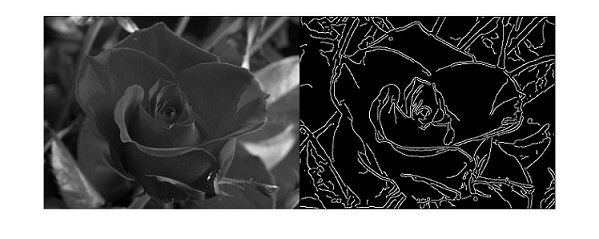
\includegraphics{images/cannyexample2}}
      \end{figure}
         
%=========================================================
\فصل*{ضمیمه}
\addcontentsline{toc}{chapter}{ضمیمه}

\clearpage
\bibliographystyle{unsrt}
\bibliography{references}

\begin{latin}
\chapter*{Abstract}

\end{latin}
\clearpage
\thispagestyle{empty}
\begin{latin}
\vspace*{-2cm}
%\[\includegraphics[width=0.2\textwidth]{arm.eps}\]
\begin{figure}
\centerline{\includegraphics{images/logo}}
\end{figure}
\vspace{0.5cm}
\begin{center}
{\large\bf  Sharif University of Technology  }\\
{\large \bf  Department of Computer Engineering}\\
\vspace{0.2cm}
{\large\bf  B. Sc. Thesis  }\\
{\large \bf  Software Engineering}\\
\vspace{1.2cm}
Title:\\
%\vspace{0.5cm}
{\Huge \bf Discrete Guassian Sampling method in lattice-based cryptography}\vspace{0.5cm}\\
Author:\vspace{0.3cm}\\
{\LARGE  \bf Mona Hadibarhaghtalab}\\
\vspace{0.5cm}
Supervisor: {\Large \bf Dr. Rasool Jalili
}\\
%Co-Supervioser: {\Large \bf Dr. Mir Omid HajiMirsadeghi 
%}\\
\vspace{1cm}
{\large \bf October 2015}
\end{center}
\end{latin}

\end{document}

